\chapter{Evaluation}
\label{cha:evaluation}
\section{Function}
The primary testing method was manual testing, which proved sufficient enough for a sole developer, however ideally, for an open-source project there would need to be tests, as new contributors would not feel confident making changes without automatic checks to see if anything got broken.
All of the functional aims and user requirements have been fulfilled. Measurements from Withings watch and Oura ring are successfully pulled into the backend in real-time as new data becomes available, accomplishing the same functionality as aggregators like Google Fit. The following is screenshot proof: Withings steps: \ref{fig:withingsSteps}, Oura steps: \ref{fig:ouraSteps} - both on a dashboard: \ref{fig:openFitCompanionSteps}. Other examples are present on the screencast.
One part of the user story for the weekly report that was not fulfilled was a comparison with other weeks, such as the green arrow if consistency improved or the red one if it got worse. 
\begin{figure}
    
    \centering
    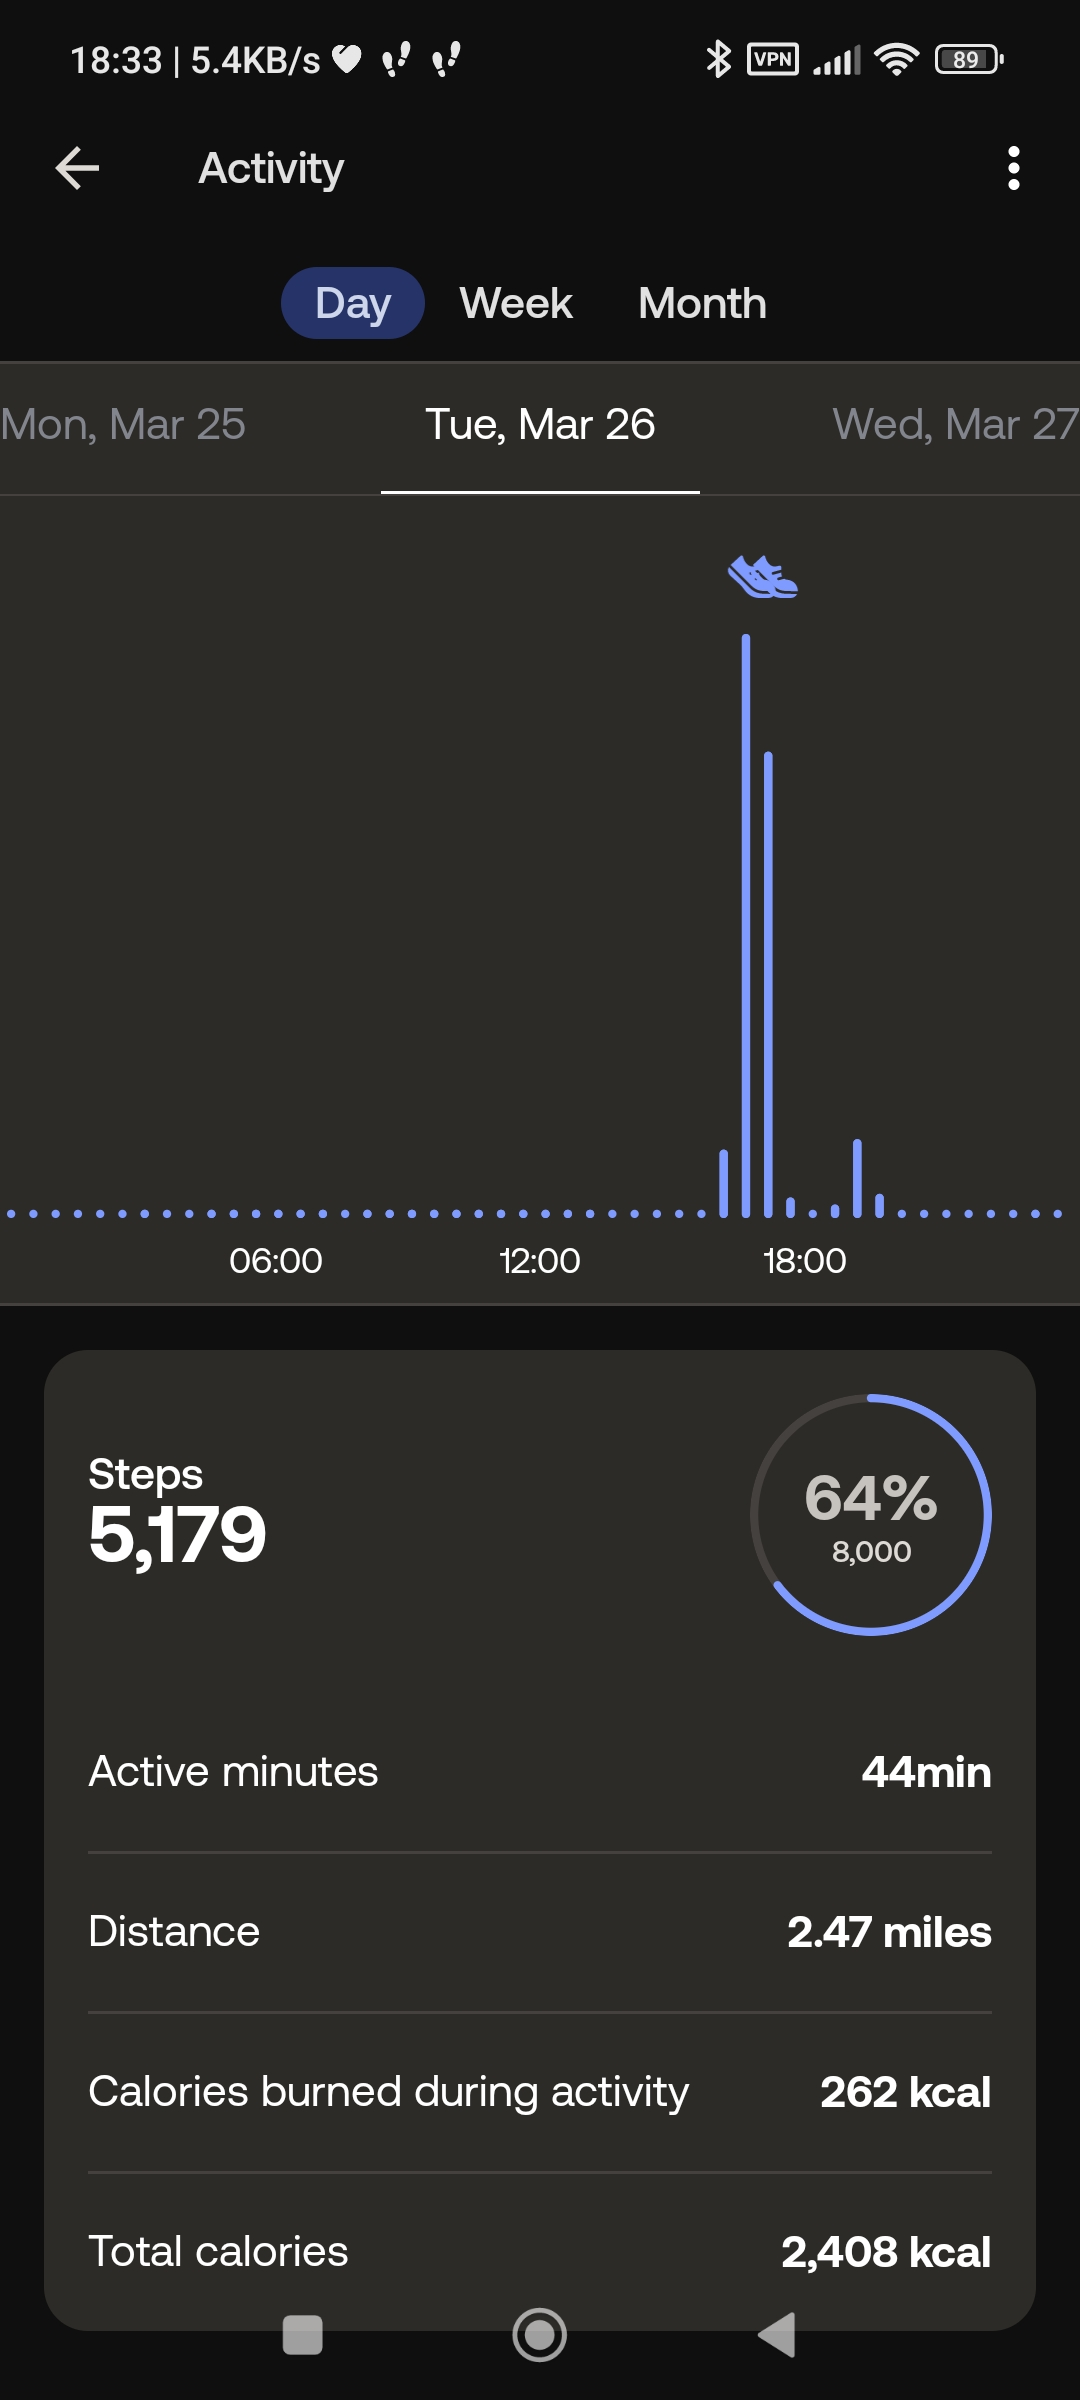
\includegraphics[width=0.5\textwidth,keepaspectratio]{../images/WithingsActivity.jpg}
    \caption{Withings Step count for 26th April}
    \label{fig:withingsSteps}
    
\end{figure}

\begin{figure}
    
    \centering
    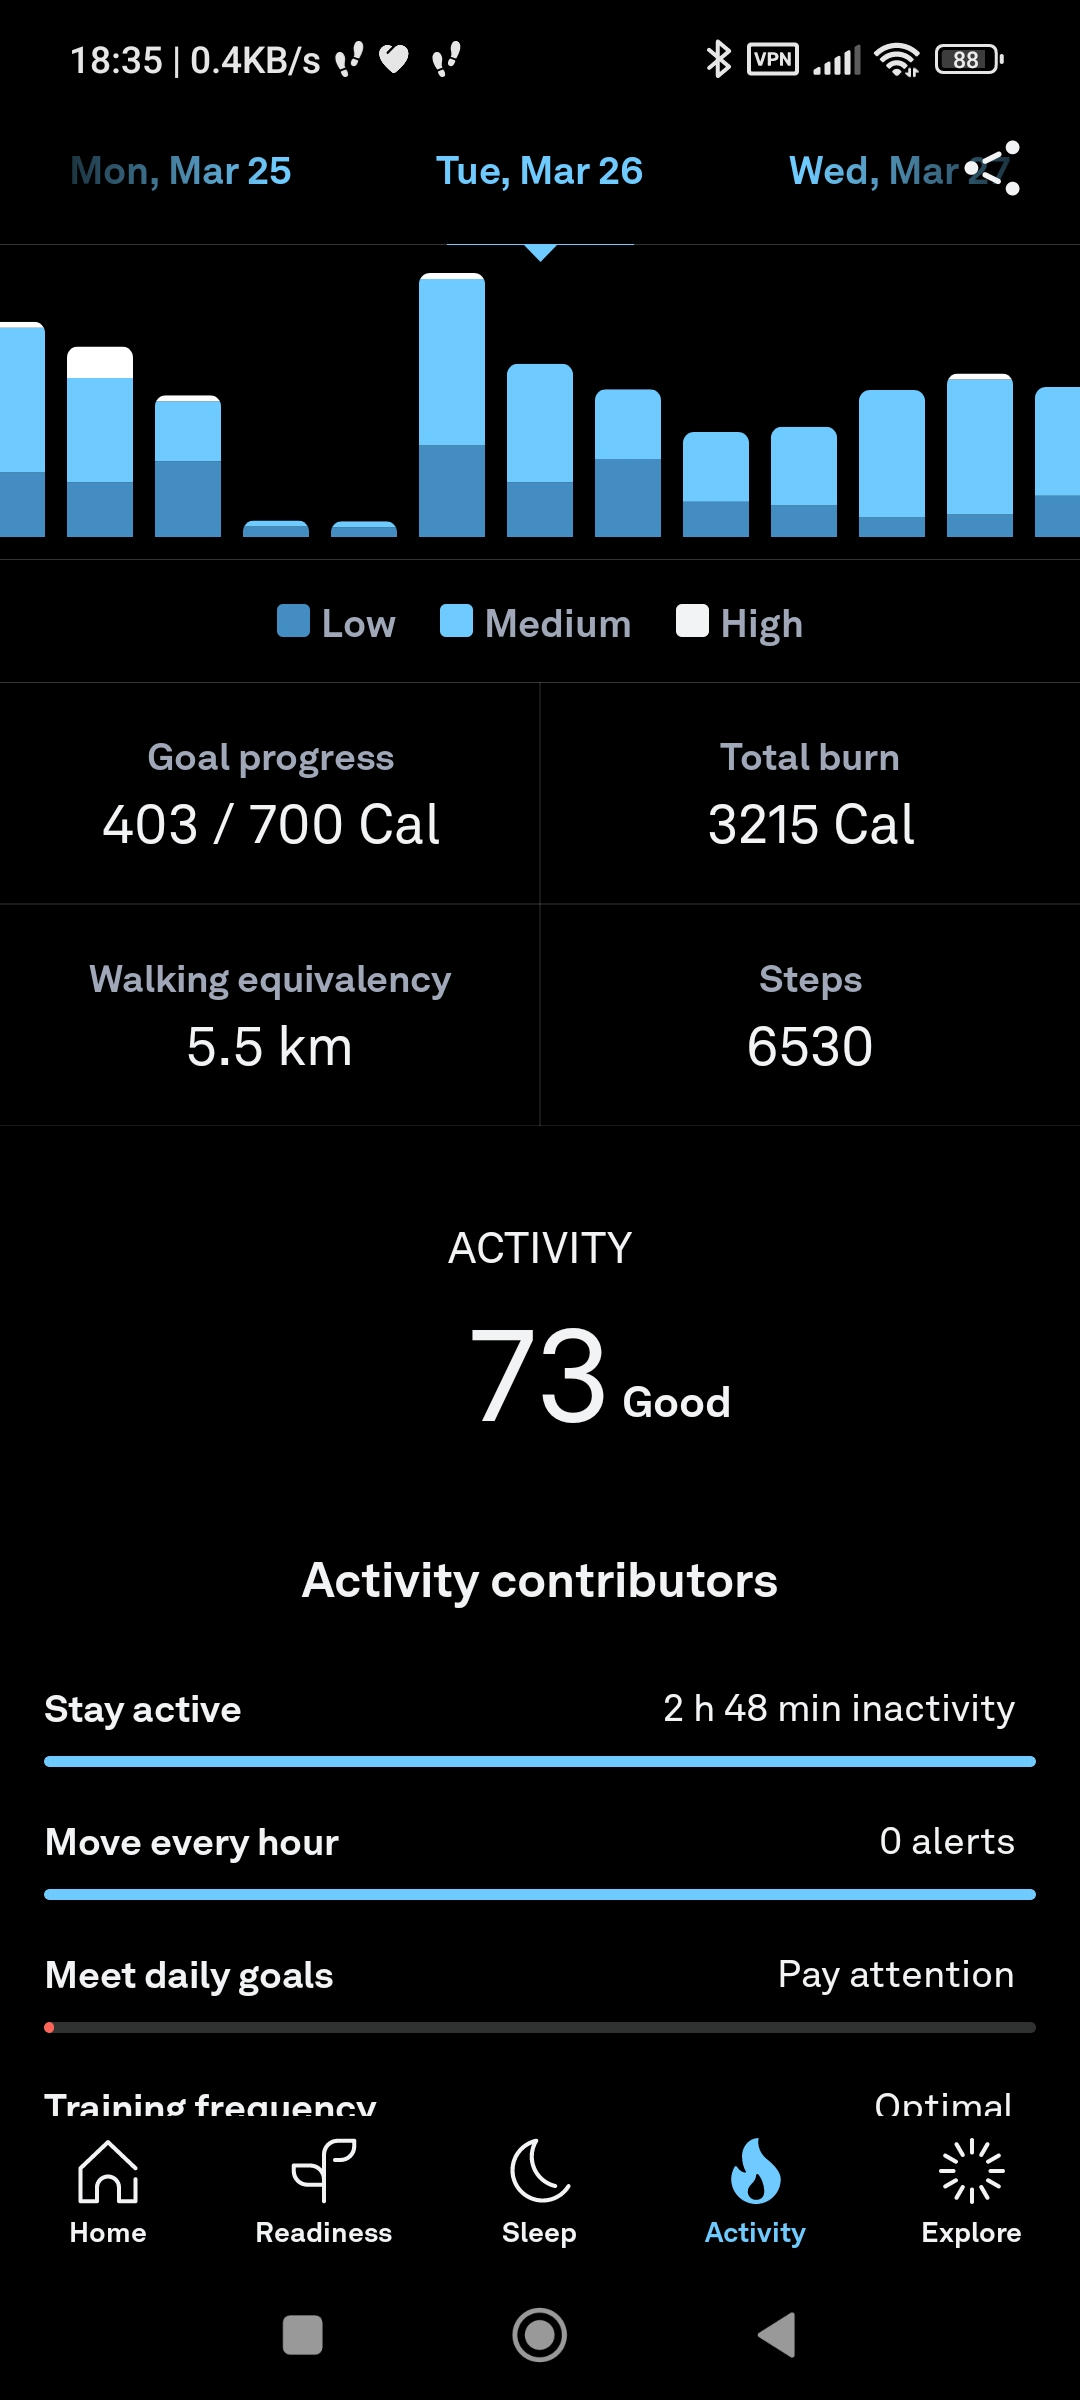
\includegraphics[width=0.4\textwidth,keepaspectratio]{../images/OuraActivity.jpg}
    \caption{Oura Step count for 26th April}
    \label{fig:ouraSteps}
    
\end{figure}
\begin{figure}
    
    \centering
    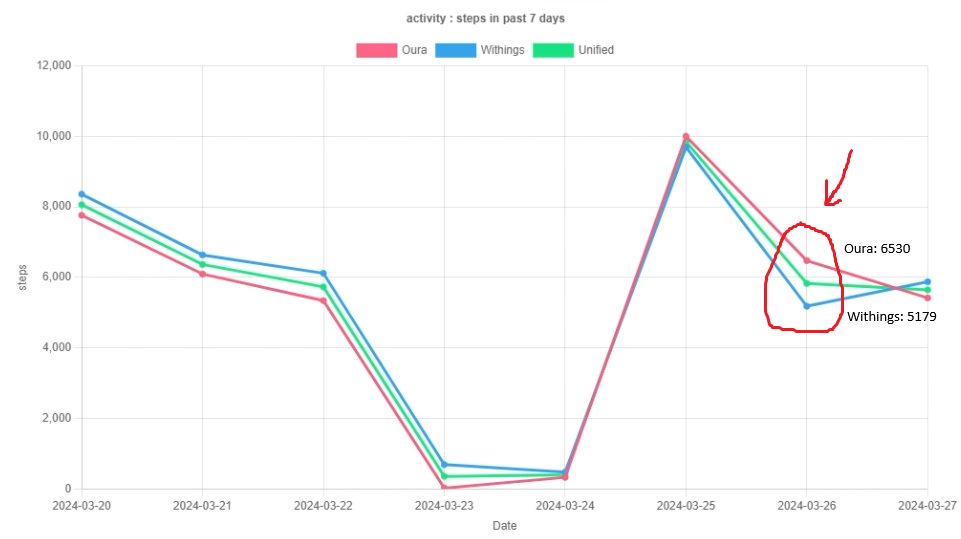
\includegraphics[width=1\textwidth,keepaspectratio]{../images/dashboard.png}
    \caption{OpenFitCompanion Step count for 26th April}
    \label{fig:openFitCompanionSteps}
    
\end{figure}

\section{Security}
\subsection{Automatic Vulnerability Scanners Testing}
Automatic web application vulnerability and penetration testing software were used to test the security of the application. The following results were obtained: 
\begin{itemize}
    \item Wapiti (Open-source): \ref{fig:wapiti} (note: screenshot is trimmed, the rest of the report showed 0 vulnerabilities)
    \item ZAP (Open-source, made by OWASP): \ref{fig:zap}
    \item Intruder (Commercial, Large-scale grade): \ref{fig:intruder}
\end{itemize}
Scanners were used to probe how a person on the internet could try to breach the website - Scanners were not run in authenticated mode, since the authentication is only possible by the owner - since there is only one user, no privilege elevation vulnerability is possible. No critical or high-risk vulnerabilities were discovered. ZAP gave false positives with hidden files, which are normal for Amplify and they don't expose any sensitive info.  Addressing interesting findings one by one: 
\begin{itemize}
    \item Clickjacking: Although no information or access is exposed, attackers may force spending OpenAI credits by masking the send prompt button - creating a lot of GPT4 generation requests. It requires a targeted attack on the owner, which is unlikely but the fix is an easy one-line change, so it should have been implemented.
    \item CSP: Only matters if the user willingly XSS infects themselves or if providers get hacked and return XSS-infected payloads. Although it is unlikely to happen, it is an easy fix and should have been implemented as well. 
    \item Strict Transport Security: The default in modern browsers is HTTPS, and if the user purposefully goes to the HTTP version, it is mostly user error, however, this may happen with less technical users. This was missed and should have been implemented.
\end{itemize}
\begin{figure}
    
    \centering
    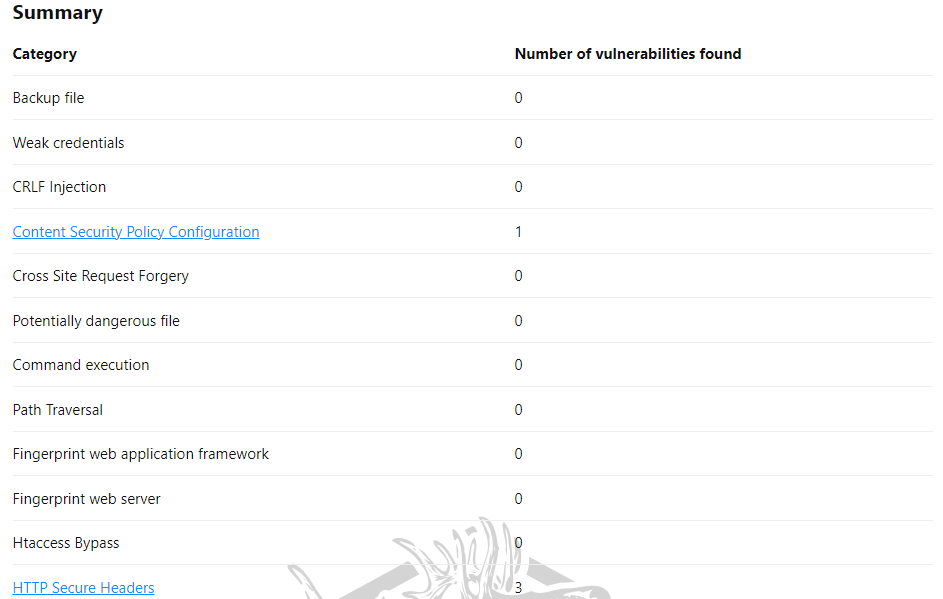
\includegraphics[width=0.9\textwidth,keepaspectratio]{../images/Wapiti.png}
    \caption{Wapiti scan result}
    \label{fig:wapiti}
    
\end{figure}
\begin{figure}
    
    \centering
    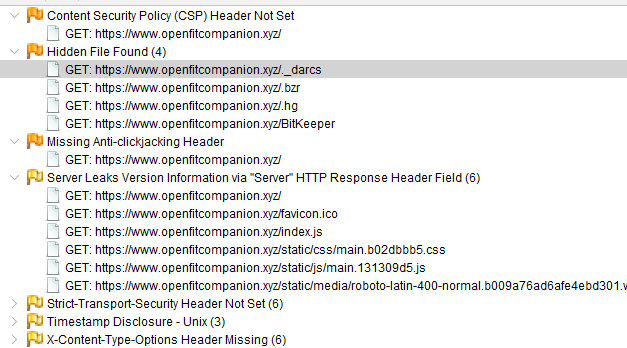
\includegraphics[width=0.8\textwidth,keepaspectratio]{../images/ZapResults.png}
    \caption{ZAP scan result}
    \label{fig:zap}
    
\end{figure}
\begin{figure}
    
    \centering
    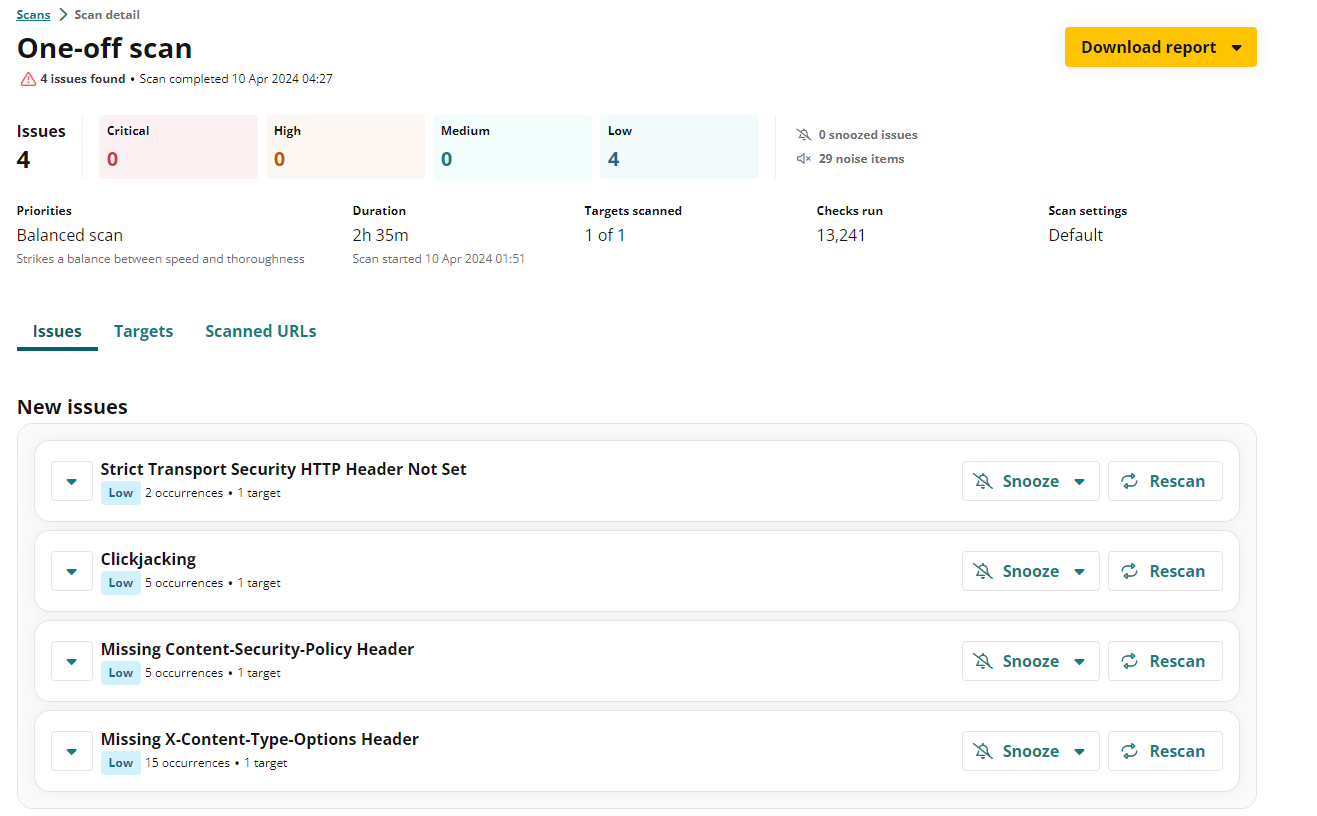
\includegraphics[width=1\textwidth,keepaspectratio]{../images/IntruderResults.png}
    \caption{Intruder scan result}
    \label{fig:intruder}
    
\end{figure}
\subsection{IAM}
AWS IAM access analyzer was used to find services that can be invoked externally: \ref{fig:awsexternal}. No issues were found, as only the entry points into the system are public. Note: test is a misnamed service for Withings notification handle and requestTokens is an OAUTH callback handler for Withings as well.

Unfortunately, there were no automatic AWS IAM role analysers for the least privilege, so it was done manually: \ref{table:IAMroles}. All roles only had the minimal necessary permissions to perform their function. 
\begin{figure}
    
    \centering
    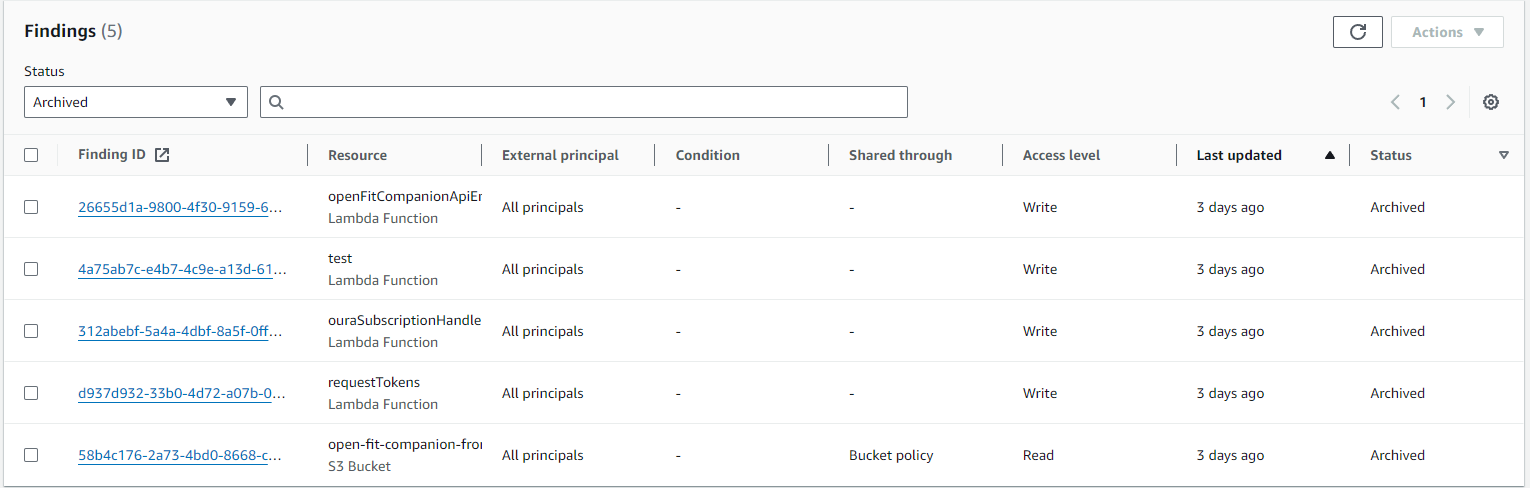
\includegraphics[width=1\textwidth,keepaspectratio]{../images/IAM_external.png}
    \caption{AWS Access analyzer - External access results}
    \label{fig:awsexternal}
    
\end{figure}
\begin{longtblr}[
    caption={IAM roles},
    label={table:IAMroles}
] {
    colspec = {|X|X|},
    rowhead = 1,
    hlines,
}
    Services & Permissions \\
    ApiEndpoint & DB: UserData: Read and Write; HealthData: Read; S3 exportBucket create object \\
    WithingsNotificationProcessor \& OuraNotificationProcessor & SNS publish \\
    ProcessNotification & DB: HealthData: Read and Write; Tokens: Read and Write; SQS: Read\\

\end{longtblr}
\section{Cost}

\subsection{Core Service}
Cost calculations were made using actual usage from February 2024, and the pricing used is also from that period. Some services like Cloudwatch (logging) or categories such as Amplify build artefacts, were used only for development and are not necessary to run the service, so they will be excluded. Let's assume that data export is done once every month. Table: \ref{table:awscost}
\begin{longtblr}[
    caption={AWS costs},
    label={table:awscost}
] {
    colspec = {|X|X|X|},
    rowhead = 1,
    hlines,
}
    Service & Usage & Cost \\
    Lambda & GB-seconds: 717 seconds; Requests: 4531 & 0.0129\$ \\
    DynamoDB & Read capacity unit hours: 2160; Write capacity unit hours: 2160; Storage: 182KB & 1.6848\$ \\
    Amplify & Data Out: 0.063GB & 0.00945\$ \\
    SNS & Requests: 810 & 0.000405\$ \\
    S3 & Storage: 0.003GB & 0.000069\$ \\

\end{longtblr}
The total per month is 1.7\$ or 1.29£. The only one that will increase with more usage is DynamoDB storage, however the health data is very light, with the entire table of 80 days weighing 120KB. AWS Always Free Tier covers all of the expenses for this usage, so actually 0£ are paid for the core application without AI. It can easily be used the same as free aggregators like Google Fit or Apple Health, but owning the data in your controlled infrastructure. However, it is worth noting that AWS can change any of the Free Tier reductions at any point, so minimising cost without it is still worth it.
\subsection{AI}
Using LLMs is where costs get dire. At the time of writing, OpenAI charges 10\$ per 1M tokens with all GPT4 models. Due to the nature of RAG, the number of tokens used for a request varies, an average number of tokens is calculated from the last 5 requests. Table: \ref{table:gptCosts} 
\begin{longtblr}[
    caption={GPT4 Costs},
    label={table:gptCosts}
] {
    colspec = {|X|X|X|},
    rowhead = 1,
    hlines,
}
    Prompt & Tokens & Cost \\
    Daily Feedback & 28643 tokens;  & 0.286\$ \\
    Activity Plan & 29566 tokens; & 0.295\$ \\
    Knowledge Retrieval & Files: 1;  & 0.2\$ \\
\end{longtblr}
So, the daily cost is 0.78\$ or 0.67£, translating to 20.15£ per month. That only accounts for automatic AI use, on-demand use through free-form chat would increase this number. 
\subsection{Commercial product comparison}
Costs are compared to other commercially available products that provide guidance in health and/or fitness, although they offer quite different degrees of personalisation, with the ones that have AI in the name offering hugely more personalised service - \ref{table:costCompare}.
\begin{longtblr}[
    caption={Cost Comparison},
    label={table:costCompare}
] {
    colspec = {|X|X|},
    rowhead = 1,
    hlines,
}
    Product & Monthly Cost \\
    OpenFitCompanion & 20.15£ (AI, rest Free Tier)  \\
    Apple Fitness+ & 9.99£ \\
    MyFitnessPal & 15.99£ \\
    EvolveAI & 19.99£ \\
    CoachifyAI & 28.49£ \\ 
    Withings+ & 8.95£

\end{longtblr}
Our product is not competitive with existing commercial products, only being cheaper than CoachifyAI. They would likely provide better quality insights due to having fine-tuned models and better rates with providers such as OpenAI, AWS, etc. To compete, our solution would need to be very cheap, like 7£ per month maximum. I suspect that token counts are so high because frequently unnecessary entries of health data are included. OpenAI says: "Retrieval currently optimizes for quality by adding all relevant content to the context of model calls. We plan to introduce other retrieval strategies to enable developers to choose a different tradeoff between retrieval quality and model usage cost". For some reason, the model includes a lot more than what is needed for the request. Researching more led to the discovery that for efficient retrieval, the data must be arranged in a specific way \cite{openForum}, with no mentions of such in the official documentation. More optimisations are needed here.
\cite{knowledgeRet}

\section{Customisability}
User requirements specified that all variables, configurations, etc should be easily customizable by a user through GUI. The following table summarises parameters in the system and whether they are fully customizable: \ref{table:customizability}.
\begin{longtblr}[
    caption={Customizability of system},
    label={table:customizability}
] {
    colspec = {|X|X|},
    rowhead = 1,
    hlines,
}
    Parameter & Customisable? \\
    MET minutes target & Yes \\
    Home equipment & Yes \\
    Athleticism level & Yes \\
    Gym days & Yes \\
    Excluded activities & Yes \\
    Daily Report notification time & No \\
    Exercise notification time & No \\
    Concentration of exercises & No \\
    
\end{longtblr}
Scheduled events such as daily report notification as well as concentration of exercises (such as more exercises in the morning please) were hard-coded, as they would require a lot more work to implement. However, all else can be modified through GUI and that information is accurately reflected in insights.
\subsection{Ease of set-up}
Ideally, even a non-technical would be able to follow easy set-up steps and have an application running in the cloud. Unfortunately, the end product can't be classified as such. Creating and modification of AWS resources mainly happened on the web console through GUI. It was done to develop features fast. However, this meant that the infrastructure would not be easily reproducible. Fortunately, there is a service - Former2 that can analyse existing resources in an AWS account and create a CloudFormation configuration file, which can be used to reproduce the same infrastructure in a brand-new account. However, the service is not perfect and trying to deploy it in a new account resulted in errors, which were not fixed by deadline. Also, the setup requires manually registering an application with Withings while Oura simply provides a personal access token. This is not something that can be fixed, as automating it is botting, which is illegal.
\subsection{Latency}
Latency can sometimes be poor. This is the latency for API response to the frontend on cold start: \ref{fig:latencyBad}, and this is the second invocation \ref{fig:latencyGood}. Latency on cold start can reach up to 2.5 seconds. This probably is not only due to Lambda cold start; DynamoDB probably also has a caching mechanism, so latency doubles up. However, on subsequent requests, the latency is satisfactory at around 200ms.   
\begin{figure}
    
    \centering
    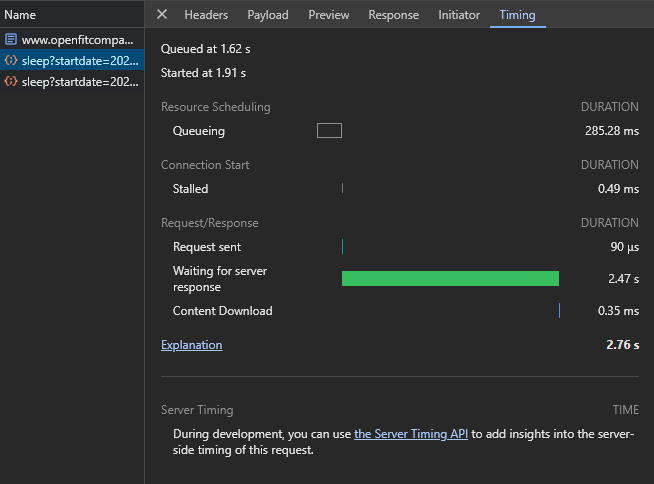
\includegraphics[width=0.8\textwidth,keepaspectratio]{../images/latencyBad.png}
    \caption{Latency on cold API function}
    \label{fig:latencyBad}
    
\end{figure}
\begin{figure}
    
    \centering
    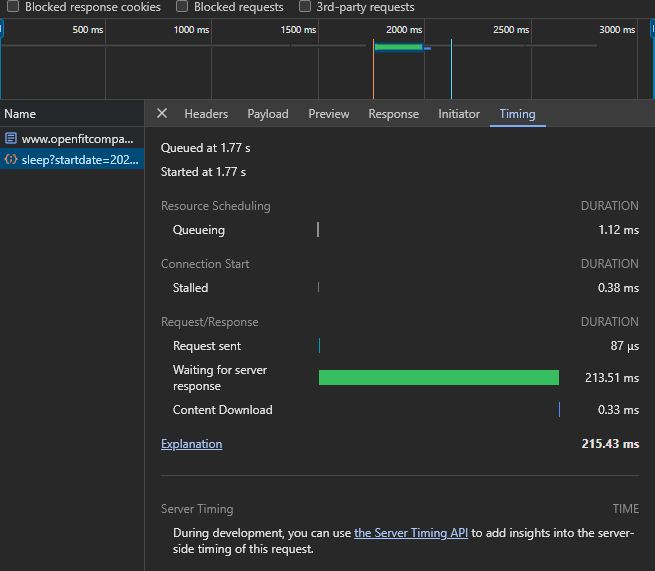
\includegraphics[width=0.8\textwidth,keepaspectratio]{../images/latencyGood.png}
    \caption{Latency on hot API function}
    \label{fig:latencyGood}
    
\end{figure}

\section{Frontend Performance \& Accessibility \& UI}
Lighthouse automated testing suite for web pages was used on every page, configured for mobile mode. Screenshot of dashboard results \ref{fig:lighthouse}. Results are collated in a table: \ref{table:lighthouse}
\begin{longtblr}[
    caption={Lighthouse testing results},
    label={table:lighthouse}
] {
    colspec = {|X|X|X|X|},
    rowhead = 1,
    hlines,
}
    Page & Performance & Accessibility & Best Practices \\
    Dashboard & 93\% & 98\% & 96\% \\
    Daily Report & 92\% & 100\% & 96\% \\
    Weekly Report & 95\% & 100\& & 96\% \\
    Profile & 93\% & 100\% & 96\% \\
    Activity Plan (largest) & 82\% & 100\% & 96\% \\
    AI Chat & 94\% & 100\% & 96\% \\

\end{longtblr}
Performance results are satisfactory, ensuring a snappy feel even when used on mobile networks. No accessibility issues were found and best practices are strictly adhered to. Unfortunately, all health data aggregators are app only, therefore it is not possible to directly compare their performance against ours; for reference, sites with dynamic content and graphs - such as Investing.com, have performance scores of around 60 (with Adblock enabled). The score drops on the Activity plan page, mainly due to exercise video examples via YouTube embeds. View window rendering may help to alleviate this, by only rendering components that are visible to the user.
\begin{figure}
    
    \centering
    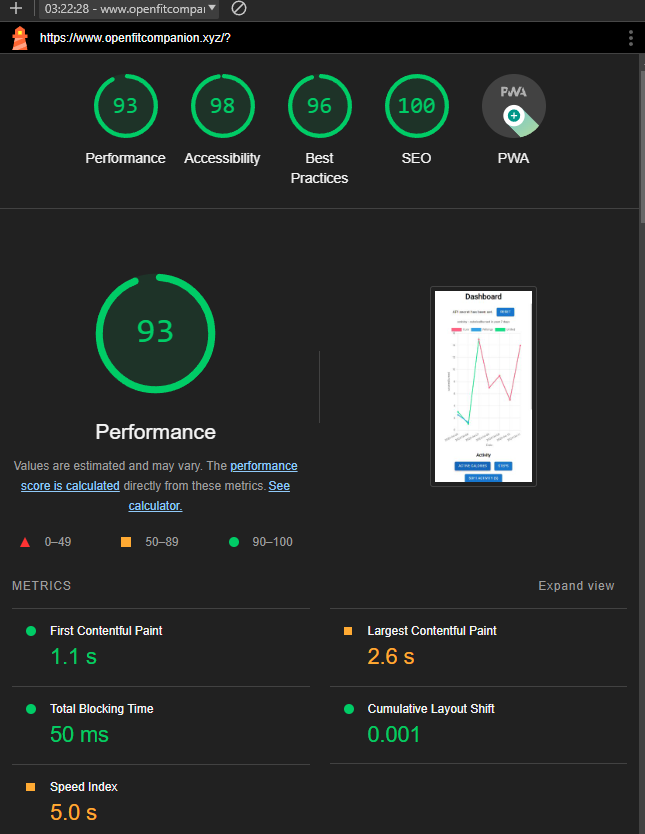
\includegraphics[width=0.75\textwidth,keepaspectratio]{../images/lightHouseMainPage.png}
    \caption{Lighthouse test result for dashboard}
    \label{fig:lighthouse}
    
\end{figure}

Each page has been evaluated for UI quality by checking if all applicable golden rules \ref{section:goldenRules} of UI are followed. For example, the profile page \ref{fig:profile} follows "Prevent errors" rule, as it uses proper input types, such as numeric only for weight field, preventing the user from entering invalid characters. However it does not follow: "Dialogs that yield closure", since no success message is displayed after form submission. Results are collated in the following table: \ref{table:goldenRulesUi}, with evaluation for each relevant rule having 3 possible values: "No", "Maybe", "Yes", with maybe used whenever it is up to the interpretation.
\begin{figure}
    
    \centering
    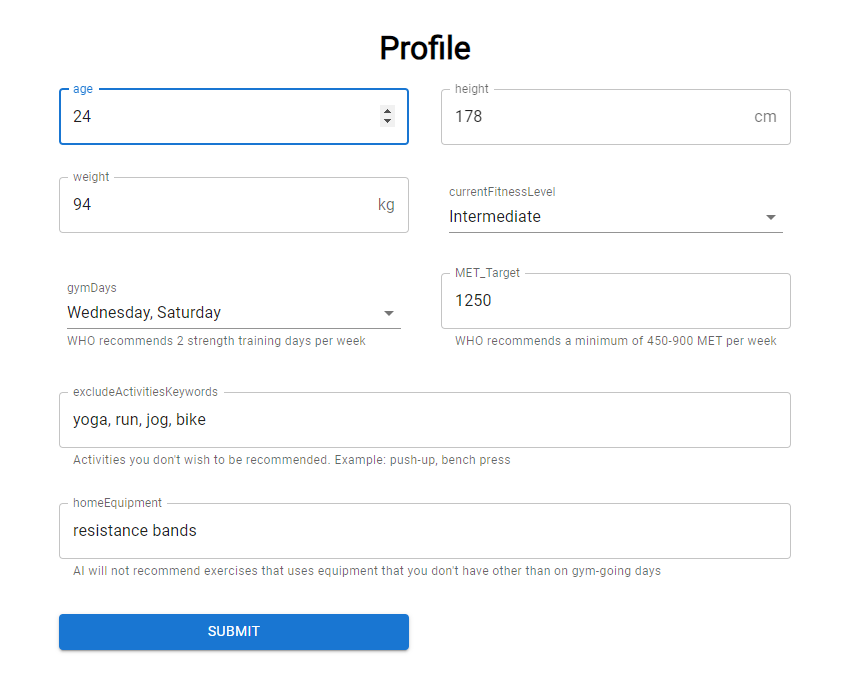
\includegraphics[width=1\textwidth,keepaspectratio]{../images/profilePage.png}
    \caption{Profile Page}
    \label{fig:profile}
    
\end{figure}
\begin{longtblr}[
    caption={Golden Rules UI evaluation results},
    label={table:goldenRulesUi}
] {
    colspec = {|X|X|},
    rowhead = 1,
    hlines,
}
    Page & Rules: Compliance \\
    Dashboard & 1: Yes; 2: Maybe; 3: Yes; 8: Yes \\
    Profile & 1: Yes; 2: Maybe; 3: Yes; 4: No; 5: Yes; 6: Yes; 8: Maybe \\
    Daily Report &  1: Yes, 2: Maybe, 8: Yes \\
    Weekly Report & 1: Yes, 2: Maybe, 8: Yes \\
    Exercise Plan & 1: Yes; 2: Maybe, 8: Maybe \\
    AI Chat & 1: Yes, 2: Maybe, 3: No, 4: No, 5: No, 6: No, 8: Yes \\

    
\end{longtblr}
To comment on a few interesting entries, universal usability compliance on any page is debatable, it can be used on any device, but there is no internationalization such as different date/calendar formats, like US "mm/dd/yyyy" date format. AI chat was the worst one, no feedback is displayed when the user submits a prompt, and only after manually refreshing the page the outcome is seen. Also no reversal: once the request is sent there is no option to cancel it.
\section{AI Insights Quality}
Providing quantifiable metrics for LLM response quality would be too complex and out of scope for this project. One good example and one bad example of insight will be provided, as well as personal thoughts about the insights after using the service as a normal user for 10 days. 
\begin{figure}
    
    \centering
    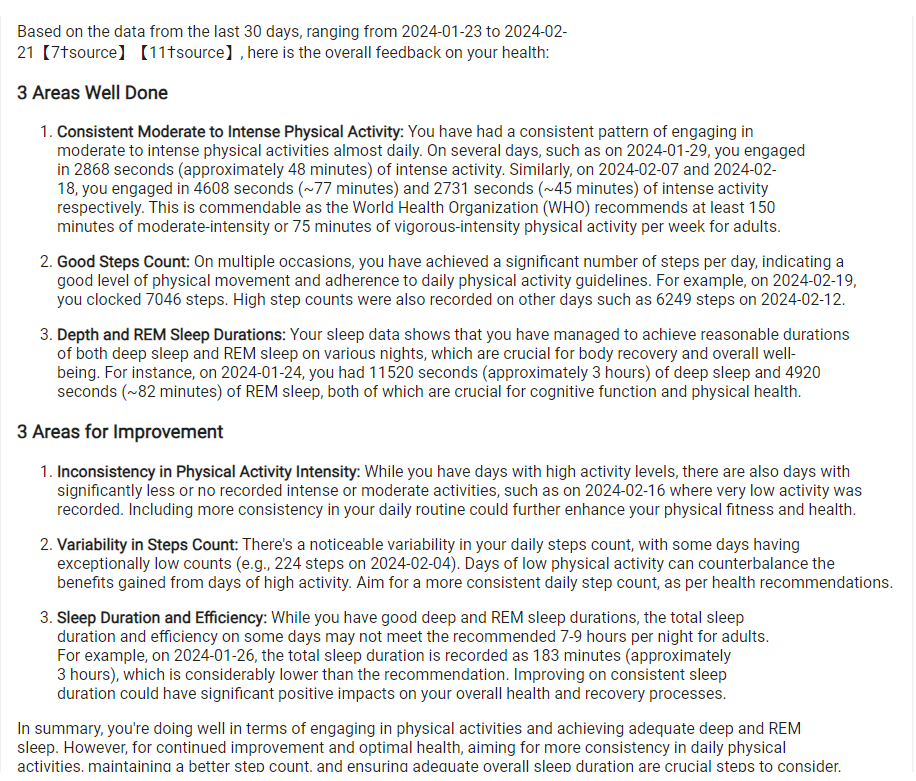
\includegraphics[width=1\textwidth,keepaspectratio]{../images/GoodAi.png}
    \caption{Good AI insight: Monthly feedback}
    \label{fig:goodAi}
    
\end{figure}
\begin{figure}
    
    \centering
    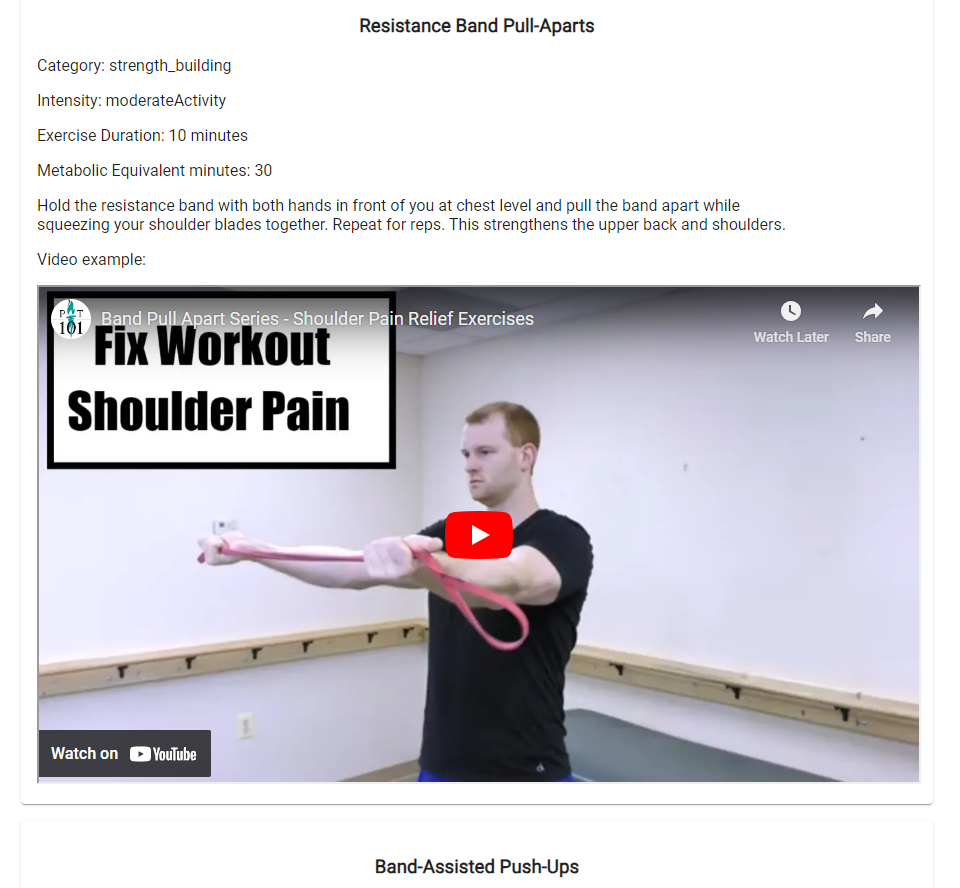
\includegraphics[width=1\textwidth,keepaspectratio]{../images/BadAi.png}
    \caption{Bad AI insight: Exercise Plan}
    \label{fig:badAi}
    
\end{figure}

A positive is LLM's ability to parse, analyse and spot some trends. A JSON file that is quite raw and unformatted is uploaded and analysed successfully by GPT4. For example, when requesting monthly feedback \ref{fig:goodAi}, it can point out variability in step count, showing on which day there were significantly fewer steps than in the general trend. It was able to distinguish between variability/consistency versus average, as it pointed out that although mean physical activity per day is high, inconsistencies are also present, which is detrimental to health. All of the findings accurately reflect reality, it does not invent numbers out of thin air, and the points made are likely something that a human fitness coach would spot as well.

One issue that wasn't solved is "obsessiveness" towards some details. For example, on non-gym days exercises should have the option to occasionally involve the user's home equipment such as resistance bands. Unfortunately, after adding this to the instructions, nearly all exercises have to do with resistance bands \ref{fig:badAi}, which gets boring. Nothing of the following worked: "mix of home equipment exercises and no equipment needed exercises", "50\% home-equipment and 50\% no equipment needed", "prioritise a variety of types of exercise", etc. The reply is always on one side of the extreme, whereas the desired result is in the middle.

Trends are often surface-level in-depth, mainly just picking out the obvious and not reading between the lines. For example, when the daily feedback pointed separately that soft activity and steps were areas to be improved, however, they are very similar; instead, it could advise going on more walks to improve both metrics at the same time, rather than improving those metrics separately. Another negative point is that developing a good prompt requires a lot of trial and error, which is expected, but there is a large cost. 40£ of personal funds were spent during development; this isn't very appealing to open-source contributors.

More investigation is required to improve pattern recognition so that insights are more useful.
\section{Comparing Devices - Discussing results}
Discussing \ref{fig:results}, to give an example of what an equivalence bound is, at 95\% confidence, if measurements are allowed to differ by more than 321 steps, then devices will be considered equal. Consequently, setting the tolerance lower than 321 will conclude that devices are different. Both devices are equivalent in steps. This is expected, as steps are not derived using biodata, but rather using dedicated hardware such as an accelerometer, so the difference should not be large. There is no confirmation from official documentation, but it is suspected that the watch simply classifies REM sleep as deep sleep, because during the same time at night it shows REM sleep in the Oura app \ref{fig:ouraRem}, while Withings has it as deep sleep \ref{fig:withingsRem}. This would essentially make sleep comparisons not valid, as they have different frameworks. The only sleep metric that is equivalent between devices is total sleep duration, although only at higher 99\% confidence. This suggests that devices might be similar for sleep tracking, but the comparison can't be made as the watch has a completely different framework with no REM sleep.  The confusing one is calories burned, which is deemed the same between the two devices, but all other activity properties are significantly different. It would make sense for calories to be different as well, as it is most likely derived from them. The watch tends to have more intense activity and the ring has more soft activity, so that overall difference balances out resulting in similar calories burned.
\begin{figure}
    
    \centering
    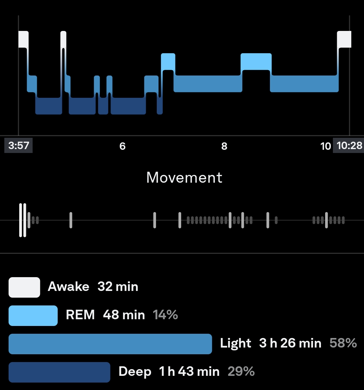
\includegraphics[width=0.7\textwidth,keepaspectratio]{../images/oura_rem.png}
    \caption{Oura app showing REM sleep between 8:18 and 8:45}
    \label{fig:ouraRem}
    
\end{figure}
\begin{figure}
    
    \centering
    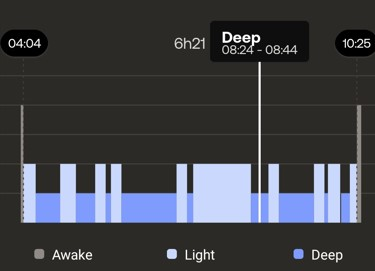
\includegraphics[width=0.7\textwidth,keepaspectratio]{../images/withings_rem.jpg}
    \caption{Withings app showing deep sleep between 8:24 and 8:44}
    \label{fig:withingsRem}
    
\end{figure}
Answering the research question, there is evidence to suggest that devices measure activity seconds of certain intensities (soft, moderate, intense) differently. All of the other metrics either show equivalence or are not directly comparable. 